\documentclass[../main.tex]{subfiles}

\begin{document}
\section{Definitions}
  \begin{itemize}
    \item Return ($G_{t}$) is the total discounted reward
    \begin{equation*}
      G_{t} = R_{t+1} + \g R_{t+2} + ... = \sum_{k=0}^{\infty}\g^{k}R_{t+k+1}
    \end{equation*}
    \item Value function: expected return starting from state $s$
    \begin{equation*}
      v(s) = \mbb{E}[G_{t}|S_{t} = s]
    \end{equation*}
    \item State value function: expected return starting from state $s$ and following policy $\pi$
    \begin{align*}
      v_{\pi}(s) &= \mbb{E_{\pi}}[G_{t}|S_{t} = s] \\
                 &= \sum_{a \in \mcal{A}} \pi(a|s) q_{\pi}(s,a)
    \end{align*}
    \item Action value function: expected return starting from state $s$, taking action $a$ and following policy $\pi$
    \begin{align*}
      q_{\pi}(s,a) &= \mbb{E_{\pi}}[G_{t}|S_{t} = s, A_{t} = a] \\
      &= \mcal{R}_{s}^{a} + \g \sum_{s' \in \mcal{S}} \mcal{P}_{ss'}^{a} v_{\pi}(s')
    \end{align*}
    \item Policy: distribution over actions given states
    \begin{equation*}
      \pi(a|s) = \mcal{P}[A_{t} = a | S_{t} = s]
    \end{equation*}
    \item Optimal state-value function : maximum value function over all polices
    \begin{equation*}
      v_{*}(s) = \text{max}_{\pi} v_{\pi}(s)
    \end{equation*}
    \item Optimal action-value function is maximum action-value function over all policies
    \begin{equation*}
      q_{*}(s,a) = \text{max}_{\pi} q_{\pi}(s,a)
    \end{equation*}
    \item Off-policy: Q-values are updated using the Q-value of the next state $s'$ and the greedy action $a'$. It estimates the return for state-action pairs assuming a greedy policy were following.
    \item On-policy: Q-values are updated using the Q-value of the next state $s'$ and the \textit{current policy's} action a'. It estimates the return for state-action pairs assuming the current policy continues to be followed.
    \item Online learning: alternate between optimizing a policy and using that policy to collect more data
  \end{itemize}

\section{Markov Decision Processes}
  \begin{itemize}
    \item describes an environment for reinforcement learning
    \item environment is fully observable
    \item the future is independent of the past given the present (e.g. $P[S_{t+1}|S_{t}] = P[S_{t+1}|S_{1}, ..., S_{t}]$)
    \item a Markov Process is a tuple $\langle \mcal{S}, \mcal{P} \rangle$
    \begin{itemize}
      \item $\mcal{S}$ is a set of states
      \item $\mcal{P}$ is a state transition probability matrix
    \end{itemize}

    \item a Markov reward process is a tuple $\langle \mcal{S}, \mcal{P}, \mcal{R}, \g \rangle$
    \begin{itemize}
      \item $\mcal{S}$ is a finite set of states
      \item $\mcal{P}$ is a state transition probability matrix
      \item $\mcal{R}$ is a reward function
      \item $\g$ is a discount factor, $\g \in [0, 1]$
    \end{itemize}

    \item a Markov decision process (MDP) is a Markov reward process with decisions, $\langle \mcal{S}, \red{\mcal{A}}, \mcal{P}, \mcal{R}, \g \rangle$
    \begin{itemize}
      \item $\mcal{S}$ is a finite set of states
      \item \red{$\mcal{A}$ is a finite set of actions}
      \item $\mcal{P}$ is a state transition probability matrix, $\mcal{P}_{ss'}^{\red{a}} = \mathbb{P}[S_{t+1} = s' | S_{t} = s, A_{t} = \red{a}]$
      \item $\mcal{R}$ is a reward function, $\mcal{R}_{s}^{\red{a}} = \mbb{E}[R_{t+1} | S_{t} = s, A_{t} = \red{a}]$
      \item $\g$ is a discount factor, $\g \in [0, 1]$
    \end{itemize}

    \item For any MDP, there exists an optimal policy $\pi_{*}$ better than or equal to all other policies, $\pi_{*} \geq \pi, \forall \pi$
    \item If we know $q_{*}(s,a)$, we immediately have the optimal policy.

    \item Bellman Optimality Equation is non-linear
    \item Many iterative solution methods:
    \begin{itemize}
      \item Value Iteration
      \item Policy Iteration
      \item Q-learning
      \item Sarsa
    \end{itemize}

  \end{itemize}

\section{Value-iteration}
  \begin{itemize}
    \item it is a method of computing an \textbf{optimal MDP policy} and its value
  \end{itemize}

\section{Q-learning}
  \begin{itemize}
    \item Off-policy Temporal Difference Control
    \item One step Q-learning:
    \item \begin{equation*}
      q(s_{t}, a_{t}) = q(s_{t}, a_{t}) + \alpha[r_{t+1} + \g \text{max}_{a}q(s_{t+1}, a) - q(s_{t}, a_{t})]
    \end{equation*}
    \item \begin{algorithm}[H]
        \SetAlgoLined
        Initialize $q(s,a) \forall s \in \mcal{S}, \forall s \in \mcal{A}, q(\text{terminal-state}) = 0$ \;
        \For {each episode} {
          Initialize s\;
          \For {each step in episode} {
            Choose $a$ from $s$ using policy derived from q (e.g. $\epsilon$-greedy)\;
            Take action $a$ and observe $r$, $s'$\;
            $q(s,a) = q(s,a) + \alpha[r + \g \text{max}_{a} q(s', a) - q(s,a)]$\;
            $s = s'$\;
          }
        }
        \caption{Q-learning}
    \end{algorithm}
  \end{itemize}

\section{Hindsight Experience Replay}

\section{RL Algorithms}
  \subsection{Taxonomy}
    \begin{itemize}
      \item
      \begin{figure}[h]
        \caption{Taxonomy of RL Algorithms}
        \centering
        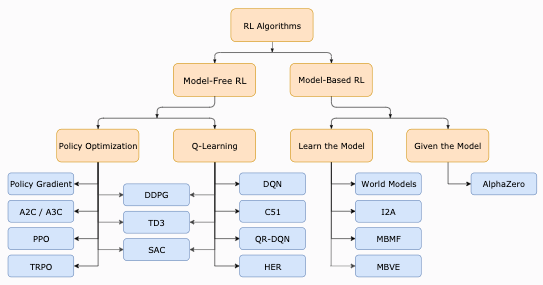
\includegraphics[width=\textwidth]{../imgs/rl_taxonomy.png}
      \end{figure}
      \item Figure from \href{https://spinningup.openai.com/en/latest/spinningup/rl_intro2.html}{OpenAI SpinningUp}
      \item Does the agent have access to a model of the environment?
      \item Having a model alows the agent to plan by thinking ahead
      \item Ground-truth model is not always available to the agent, must learn model from experience
      \item In model-free there are two main approaches for training agents: policy optimization and q-learning
      \item Policy optimization
      \begin{itemize}
        \item Represents the policy as $\pi_{\theta}(a|s)$ and optimize the parameters $\theta$ by gradient ascent on $J(\pi_{\theta}$
        \item The optimization is almost always performed on-policy
        \item Also learn an approximator $V_{\phi}(s)$
        \item Directly optimizes for the thing that you want**
      \end{itemize}
      \begin{itemize}
        \item Q-learning learns an approximator $Q_{\theta}(s,a)$ for the optimal action-value function
        \item Q-learning is almost always performed off-policy, update uses data collected at any point during training
        \item $a(s) = \text{argmax}_{a}Q_{\theta}(s,a)$
        \item Indirectly optimization, tens to be less stable, more sample efficient because they can reuse data more effectively
      \end{itemize}
    \end{itemize}
  \subsection{Policy Gradients}
    \begin{itemize}
      \item Maximize the expected return $J(\pi_{\theta}) = E_{\tau \sim \pi_{\theta}}[R(\tau)]$
      \item Optimize policy: $\theta_{k+1} = \theta_{k} + \alpha \nabla_{\theta}J(\pi_{\theta})|_{\theta_{k}}$
      \item Gradient of policy performance $\nabla_{\theta}J(\pi_{\theta})$ is the policy gradient
      \item $\nabla_{\theta}J(\pi_{\theta}) = E_{\tau \sim \pi_{\theta}}[\sum_{t=0}^{T} \nabla_{\theta} \text{log} \pi_{\theta}(a_{t}|s_{t})R(\tau)]$
      \item This is the grad log probability and since it is an expectation, we can estimate it with a sample mean by collecting a set of trajectories
      \item The "loss" for policy gradient algorithm is not the same loss in the typical sensen from supervised learning
      \item Loss doesn't measure performance, it doesn't mean anything. It is possible to have low loss and have poor policy performance, this is due to policy overfitting to a batch of data
      \item EGLP or Expected Grad-Log-Prob Lemma states that $E_{x \sim P_{\theta}}[\nabla_{\theta} log P_{\theta}(x)] = 0$
      \item Reward-to-go policy gradient, we only care about the reward that came after taking an action
      \item Past rewards add noise to sample estimates of the policy gradient
      \item EGLP lemme implies that we can add/subtract any function $b$ that only depends on the state from the policy gradient without changing its expectation (this is called a baseline)
      \item Results in faster and more stable policy learning
      \item Common baselines:
      \begin{itemize}
        \item $\Phi_{t} = R(\tau)$
        \item $\Phi_{t} = \Sigma_{t'=t}^{T}R(s_{t'}, a_{t'}, s_{t'+1})$
        \item $\Phi_{t} = \Sigma_{t'=t}^{T}R(s_{t'}, a_{t'}, s_{t'+1}) - b(s_{t})$
        \item $\Phi_{t} = Q^{\pi_{\theta}}(s_{t}, a_{t})$ (on-policy action-value function)
        \item $\Phi_{t} = A^{\pi}(s_{t}, a_{t})$ (advantage function, describes how much better or worse an action is compared to other actions)
      \end{itemize}
      \item Baseline is often approximated using a neural network that is updated concurrently wiht the policy using a mean-squared error

    \end{itemize}

  \subsection{Deep Deterministic Policy Gradient (DDPG)}
    \begin{itemize}
      \item
    \end{itemize}


\section{Batch/Offline Reinforcement Learning}
  \begin{itemize}
    \item Most of RL algorithms assume that an agent interacts with an online environment or simulator and learns from its own collected experience. This is expensive and often requires a high-fidelity simulator which can be hard to build
    \item Offline RL addresses the problem of learning a policy from a fix set of trajectories, without any further interaction with the environment
    \item In principle, off-policy algorithm can learn from data collected by any policy
    \item Recent work shows that standard off-policy deep RL algorithms diverge in offline setting
    \item Removes design of replay buffer and exploration
    \item Challenging due to distribution mismatch between current policy and offline data collection policy
    \item Datasets:
    \begin{itemize}
      \item D4RL
      \item Developed tasks that reflect both real-world dataset challenges and real-world applications
      \item Autonomous driving, robotics, and other domains
    \end{itemize}
    \item Batch RL algorithms
    \begin{itemize}
      \item Quantile Regression DQN (QR-DQN)
      \item Random Ensemble Mixture {REM}
      \item Batch Constrained Deep Q-learning (BCQ)
    \end{itemize}

    \item Batch Constrained deep Q-learning (BCQ) \cite{bcq}
    \begin{itemize}
      \item Run normal Q-learning but in the maximization step, instead of considering max over all possible actions, only consider actions $a'$ such that $(s',a')$ actually appear in the batch of data
      \item Train a \textit{generative model} - variational autoencoder - to generate actions that are likely to be from the batch
      \item Also a \textit{perturbation model} to perturb the actions
    \end{itemize}
  \end{itemize}

\section{Curiosity Driven Exploration}

\section{Inverse Reinforcement Learning}

\section{General tips when using RL}
\begin{itemize}
  \item Notes taken from the \href{https://stable-baselines.readthedocs.io/en/master/guide/rl_tips.html}{stable-baselines documentation}
  \item Data in RL for training an agent is collected through interactions with the environment
  \item This dependences can lead to vicious circle, if the agent collects poor data, it will not improve and keep exploring bad trajectories
  \item Algorithms are dependent on hyperparameters
  \item Normalize input to agent and use common preprocessing techniques (e.g. frame-stack, etc)
  \item Model-free RL algorithms are usually \textit{sample inefficient}
  \item Expert knowledge is often needed to design adequate reward function
  \item Unstable training, often huge drops in performance especially in DDPG. Methods to remedy this include TD3, TRPO, PPO, etc
  \item Most algorithms use exploration noise, need a separate test environment to evaluate agent at test time
  \item Some policies are stochastic by default (e.g. A2C or PPO)
  \item DQN only supports discrete actions, SAC is restricted to continuous actions
  \item Also depends on whether you want to parallelize your training
  \item Keep action space in range $[-1, 1]$ and symmetrical, used in Gaussian policies
\end{itemize}

\end{document}